\PassOptionsToPackage{table}{xcolor}
\documentclass{article}
\usepackage[colorlinks]{hyperref}
\usepackage[margin=1.25in]{geometry}
\usepackage{amsmath,amssymb,amsthm,booktabs,tikz}
\usepackage[final]{microtype}
\usepackage{libertine}
\usepackage[varqu]{zi4}
\usepackage[libertine]{newtxmath}
\usepackage[T1]{fontenc}
\usepackage[utf8]{inputenc}
\usepackage{tabto}
\usepackage[normalem]{ulem}

\usetikzlibrary{shapes.multipart}

% Seven colors safe for use color blindness.
% Colors taken from doi:10.1038/nmeth.1618.
\definecolor{cbOrange}{RGB}{230,159,0}
\definecolor{cbSkyBlue}{RGB}{86,180,233}
\definecolor{cbBluishGreen}{RGB}{0,158,115}
\definecolor{cbBlue}{RGB}{0,114,178}
\definecolor{cbVermillion}{RGB}{213,94,0}
\definecolor{cbReddischPurple}{RGB}{204,121,167}
\definecolor{cbYellow}{RGB}{240,228,66}

\theoremstyle{definition}
\newtheorem{problem}{Problem}
\newenvironment{questions}{\begin{enumerate}
\renewcommand{\theenumi}{P\arabic{problem}.\arabic{enumi}}}{\end{enumerate}}
\newcommand{\HL}[1]{\textcolor{cbReddischPurple}{#1}}

\newcommand{\abs}[1]{\lvert #1 \rvert}
\newcommand{\OOG}[1]{\mathord{\sim}#1}
\DeclareMathOperator{\bdiv}{div}

\newcommand{\BigO}[1]{\mathcal{O}\left(#1\right)}
\newcommand{\BigOmega}[1]{\Omega\left(#1\right)}
\newcommand{\BigTheta}[1]{\Theta\left(#1\right)}


\newcommand{\True}{\texttt{true}}
\newcommand{\False}{\texttt{false}}

%% Tikz
\usepackage{tikz}
\usetikzlibrary{arrows.meta,calc,decorations.pathreplacing,shapes.geometric,shapes.multipart,overlay-beamer-styles}
\tikzset{
    >=Stealth,
    dot/.style={circle,scale=0.35,draw=black,fill=black},
    stacked/.style={above,rectangle split,draw,rectangle split parts=#1,font=\strut,rectangle split part fill={none,black!10}},
    centered/.append style={align=center}
}


% Algorithm
\usepackage{algorithmic}
\newcommand{\GETS}{:=}
\newcommand{\VAR}[1]{\textit{#1\/}}
\newcommand{\AName}[1]{\textsc{#1}}
\renewcommand{\algorithmicrequire}{\textbf{Input:}}
\renewcommand{\algorithmicensure}{\textbf{Result:}}
\newcommand{\CMT}[1]{\text{``#1''}}
\renewcommand{\algorithmiccomment}[1]{\CMT{#1}}
\newcommand{\INV}[1]{\emph{inv: } #1}
\newcommand{\VF}[1]{\emph{bf: } #1}
\makeatletter
\newlength{\Algo@MyTabLength}
\newcommand{\AlgoTabTo}[1]{%
    \setlength{\Algo@MyTabLength}{#1}%
    \addtolength{\Algo@MyTabLength}{-\ALC@tlm}%
    \tabto{\Algo@MyTabLength}%
}
\newenvironment{myonlyalgo}[1][0]{
    \vskip 5pt
    \hrule
    \smallskip
    \begin{algorithmic}[1]
    \setcounter{ALC@line}{#1}
}{
    \end{algorithmic}
    \hrule
    \vskip 5pt
}
\newenvironment{myalgo}[2][0]{
    \vskip 5pt
    \hrule
    \smallskip
    \noindent{\textbf{Algorithm} #2\textbf{:}}
    \begin{algorithmic}[1]
    \setcounter{ALC@line}{#1}
}{
    \end{algorithmic}
    \hrule
    \vskip 5pt
}







%% Metadata
\newcommand{\Assignment}[1]{
    \title{\vskip-2em%The standard article.cls package puts 2em whitespace on top of the title, undo this.
           Assignment #1\\{\Large SFWRENG 2CO3: Data Structures and Algorithms--Winter 2023}}}
\newcommand{\Deadline}[1]{
    \author{Deadline: #1}
}
\date{{\normalsize
    Department of Computing and Software\\
    McMaster University
}}

\newcommand{\Warning}[1]{\textbf{\textcolor{red!80!black}{#1}}}
\renewcommand{\labelitemi}{$\blacktriangleright$}

\newcommand{\DEFAULTMSG}{
Please read the \emph{Course Outline} for the general policies related to assignments.
\begin{center}
\Warning{Plagiarism is a \underline{\textit{\vphantom{y}serious academic offense}} and will be handled accordingly.}\\
\Warning{All suspicions will be reported to the \underline{\textit{Office of Academic Integrity}}\\(in accordance with the \href{https://secretariat.mcmaster.ca/app/uploads/Academic-Integrity-Policy-1-1.pdf}{Academic Integrity Policy}).}
\end{center}

This assignment is an \emph{individual} assignment: do not submit work of others. All parts of your submission \emph{must} be your own work and be based on your own ideas and conclusions. Only \emph{discuss or share} any parts of your submissions with your TA or instructor.  You are \emph{responsible for protecting} your work: you are strongly advised to password-protect and lock your electronic devices (e.g., laptop) and to not share your logins with partners or friends! If you \emph{submit} work, then you are certifying that you have completed the work for this assignment by yourself. By submitting work, you agree to automated and manual plagiarism checking of all submitted work.

\emph{Late submission policy}. Late submissions will receive a late penalty of 20\% on the score per day late (with a five hour grace period on the first day, e.g., to deal with technical issues) and submissions five days (or more) past the due date are not accepted. In case of technical issues while submitting, contact the instructor \emph{before} the deadline.}

\newcommand{\SUBMITMSG}{\section*{Assignment Details}
Write a report in which you solve each of the above problems. Your submission:
\begin{enumerate}
\item must be a \texttt{PDF} file;
\item must have clearly labeled solutions to each of the stated problems;
\item must be clearly presented;
\item must \emph{not} be hand-written: prepare your report in \LaTeX{} or in a word processor such as Microsoft Word (that can print or exported to \texttt{PDF}).
\end{enumerate}
\Warning{Submissions that do not follow the above requirements will get a grade of zero.}}

\newcommand{\DEFAULTGRADING}{\section*{Grading}
Each problem counts equally toward the final grade of this assignment.
}


\Assignment{4}
\Deadline{March 19, 2023}
\begin{document}
\maketitle
\DEFAULTMSG{}

\begin{problem}
Consider a directed graph $\Graph = (\Nodes, \Edges)$. Breadth-first search and depth-first search both have a runtime complexity of $\OOG{\abs{\Nodes} + \abs{\Edges}}$ if we represent the graph with an adjacency list.
\begin{questions}
\item What is the runtime complexity of breadth-first search and depth-first search when we use the matrix representation? Explain your answer.

For BFS, we typically use a queue to store the vertices to be 
processed. In each iteration, we remove a vertex from the front 
of the queue, add its neighbors to the back of the queue if they 
have not been visited yet, and mark the removed vertex as visited.
 To determine the neighbors of a vertex, we need to examine the
  corresponding row of the adjacency matrix. Thus, for each 
  vertex, we need to scan the corresponding row of the adjacency
   matrix to find its neighbors. Since there are $|N|$ vertices, 
   each with $|N|$ entries in the adjacency matrix, the time 
   complexity of BFS using the adjacency matrix representation 
   is $O(|N|^2)$.

For DFS, we typically use a stack to store the vertices to 
be processed. In each iteration, we remove a vertex from the 
top of the stack, add its unvisited neighbors to the stack, and 
mark the removed vertex as visited. To determine the neighbors 
of a vertex, we need to examine the corresponding row of the 
adjacency matrix. Thus, for each vertex, we need to scan the 
corresponding row of the adjacency matrix to find its neighbors. 
Since there are $|N|$ vertices, each with $|N|$ entries in the
 adjacency matrix, the time complexity of DFS using the adjacency 
 matrix representation is also $O(|N|^2)$.

\item Consider the \emph{ordered edge list} representation that represents a graph by an \emph{ordered} array $A$ that holds $\abs{\Edges}$ edges. The order of edges is as follows: edge $(n_1, m_1) \in A$ comes before $(n_2, m_2) \in A$ if $\ID{n_1} < \ID{n_2}$ or if $\ID{n_1} = \ID{n_1} \land \ID{m_1} \leq \ID{m_2}$. What is the runtime complexity of breadth-first search and depth-first search when we use the \emph{ordered edge list} representation? Explain your answer.


In the ordered edge list representation, since edges are sorted, we know all edges that start at $n_1$ will be at the start of the array, followed by $n_2$ and so on. We can then use binary search to find the first edge of the list of edges that start at $n_x$ where x is the node number. 

For BFS, we know that we traverse every node once and every edge once (covered in class). Basically, we start by visiting the start node and then all its neighbours. To visit its neighbours, we need to search for the edges that have the starting node as the first node in the tuple. To find these nodes, it takes $\OOG{log_2{|E|}}$ time where the length of the list to search is $|E|$. We repeat this process for every node, meaning we visit every node once and every edge once and need to call a $\OOG{log_2{|E|}}$ operation once per node. This gives a complexity of $\OOG{|N|log_2|E| + |E|}$.

For DFS, we also know that we traverse every node and edge once. We do this by starting at the start node and recursively visiting all its neighbours. Again, to visit the neighbours will require to find the edges in the ordered list, which requires the binary search of $\OOG{log_2{|E|}}$. We repeat this process for all nodes that are visited, thus meaning we use the binary search once per node. Since this is the case, the overall runtime complexity is also $\OOG{|N|log_2|E| + |E|}$ as we traverse every node and edge once and for every node, need to perform a $\OOG{log_2{|E|}}$ complexity search.

\end{questions}
\end{problem}

\begin{problem}
Consider a directed acyclic graph $\Graph = (\Nodes, \Edges)$ with a source node $m \in \Nodes$ and target node $n \in \Nodes$.
\begin{questions}
\item Provide an algorithm that computes the number of paths starting at $m$ and ending at $n$.

Assuming an adjacency list representation of the graph.

\begin{myalgo}{\AName{DFS}($\VAR{start},\VAR{dest},\VAR{storedPaths}$)}
  \IF{$\VAR{start}=1$}
    \RETURN 1
  \ENDIF
  \STATE $path = 0$
  \FOR{$(n, m) \in \Edges$}
    \IF{$(storedPaths.containsKey(n))$}
      \STATE $path += storedPaths.get(n)$
    \ELSE{}
      \STATE $\VAR{paths} += $\AName{DFS}($\VAR{start},\VAR{dest},\VAR{storedPaths}$)
    \ENDIF
  \ENDFOR
  \STATE $storedPaths.putIfAbsent(v, path)$
  \RETURN $paths$
\end{myalgo}

Call this via 

\begin{myalgo}{\AName{Main}()}
  \STATE $graph \GETS new Graph()$  \COMMENT{initialized graph with edges and nodes already set}
  \STATE $Map<Integer, Integer> storedPaths = new HashMap<>()$
  \PRINT \AName{DFS}($m, n, storedPaths$)
\end{myalgo}

Graph representation: adjacency list representation. The algorithm runs DFS from the start node. For each node in its adjacency list (neighbours), it runs another DFS. This happens recursively.
This algorithm still goes over what is considered a "marked node" in normal DFS as we want to account for every single path, not only unique ones. Each DFS counts the number of paths to the destination node by summing the number of paths to the destination node all of its children have.
The base case is when reaching the destination node, we have 1 path. Using this recursion, we can sum all the paths to the destination node and return that.
Theoretically, this algorithm starts at the destination node and tracks back counting all the paths from the next parent node to the destination node, and continues until reaching the start node.

As I use dynamic programming to keep track of the solution to "subproblems" (a subproblem being finding the paths to the destination node from specific node), we only ever need to compute the number of paths from a single node to the destination once. After that we can fetch that result from the storedPaths map.
This means that for every node, we perform a DFS. We know DFS using adjacency list representation is $\OOG{|N| + |E|}$, so if we do this for each node, the complexity is $\OOG{|N|^2 + |N||E|}$

\item We say that the directed acyclic graph $\Graph$ has a \emph{bottleneck} if there is a node $b$, distinct from source $m$ and target $n$, such that all paths from $m$ to $n$ go through node $b$. Write an algorithm that returns $\True$ if  and only if $\Graph$ has such a bottleneck. You may assume that there is at-least one path from $m$ to $n$.

\begin{myalgo}{\AName{Bottleneck}($\VAR{m},\VAR{n}$)}
  \STATE $G = Graph(N,E)$  \COMMENT{Initialized graph with all nodes N and edges E}
  \STATE $S = G.DFS(m)$ \COMMENT{All nodes reachable from m}
  \STATE $G_{rev}(N,E_{rev}) = (N, {e \in G | (n_1,n_2) \in E : (n_2,n_1)})$  \COMMENT{Same graph, but with all edges flipped}
  \STATE $T = G_{rev}.DFS(n)$ \COMMENT{All nodes that can reach n}
  \STATE $B = Intersection(S,T)$ \COMMENT{All nodes that are reachable from m and can reach n}
  
  \STATE $TS = TopologicalSort(B)$

  \STATE $Q = array$ \COMMENT{array of all inspected nodes}
  \STATE $Q.add(m)$
  \FOR{$h \in TS \: \: \&\& \: \: h \:!= m \: \: \&\& \: \: h \:!= n$} 
    \STATE $Q.add(h)$
    \FOR{all nodes y after h in TS}
      \IF{$(y,z) \in E_{rev} \: \: \&\& \: \: Q.contains(z)$}
        \STATE continue (skip this iteration of outer FOR loop) 
        \STATE \COMMENT{h can't be a bottleneck since an element before h points to one after it}
      \ENDIF
    \ENDFOR
    \RETURN True  \COMMENT{There are no nodes before h that point to nodes after h}
  \ENDFOR
  \RETURN False
\end{myalgo}

I am using adjacency list representation again.

In general, I get all nodes that are reachable from m and can reach n. These are all nodes that must be part of a path from m to n. Then sorting them topologically, I can get the order in which all nodes are placed in the graph. We know that any node a with an outgoing edge to node b must be before node b.
For a bottleneck to exist, there must be a node h such that all nodes after it in topological order cannot have an ingoing edge from an edge before node h. If so, there is a path that goes around node h. That way, we can check that all nodes after node h have no ingoing edges before it by using $G_{rev}$, which is a graph where ingoing nodes become outgoing and vise versa.
If there is one, we can skip to the next node in TS since we know h isn't a bottleneck. If there isn't one after checking all nodes after h, we know there is a bottle neck since no path from m to n goes around h.

DFS on line 2: Is a $\OOG{|N|+|E|}$ as it is a normal DFS where we keep track of the nodes reachable from m and return them. As mentioned in lecture, DFS is $\OOG{|N|+|E|}$.

Reversing the edges on line 3: Is a $\OOG{|E|}$ as you need to swap the nodes for every edge.

DFS on line 4: With the reverse graph, do the same as line 2 where you find all reachable nodes. This will get all nodes that can reach n in $\OOG{|N|+|E|}$.

Intersection on line 5: Goes through all of $S$ and $T$ and adds nodes that are in both sets. This is $\mathcal{O}(\OOG{|N|})$ as worst-case, all nodes are in both sets, so we must traverse the sets fully.

Topological sorting on line 6: This costs $\OOG{|N| + |E|}$ as seen in class.

The nested for loop starting on line 9: Goes through all nodes in TS once (except m and n), and for each node, traverses all nodes after it. This is $\OOG{|N|^2}$ worst case as TS might contain every node in the graph.

Looking at all the complexities above, $\OOG{|N|^2}$ seems to be the largest time complexity as $|E|$ is upper bounded by $|N|^2$. Therefore, my algorithm is $\OOG{N^2}$ complexity.




\end{questions}
For each question, explain why your algorithm is correct, what the complexity of your algorithm is, and which graph representation you use.
\end{problem}

\begin{problem}
Let $n$ be a positive integer and consider two $n \times n$ matrices $M_1$ and $M_2$. The \emph{Boolean matrix product} of $M_1$ and $M_2$, denoted by $M' \GETS M_1 \otimes M_2$, is the $n \times n$ matrix $M'$ in which $M'[i, j]$ is:
\[ M'[i, j] = (M_1[i, 0] \land M_2[0, j]) \lor (M_1[i, 1] \land M_2[1, j]) \lor \dots \lor (M_1[i, n-1] \land M_2[n-1,j]). \]

Now consider a directed graph $\Graph = (\Nodes, \Edges)$ implemented via the matrix representation $M$ with $n = \abs{\Nodes}$.
\begin{questions}
\item Let $M' = M \otimes M$. What does the value $M'[i,j]$ represent (when is it $\True$ and when is it $\False$)?

The value $M'[i, j]$ represents whether there exists a path of length 2 from node $i$ to node $j$ in the directed graph G = (N, E) represented by matrix M.

In other words, $M'[i, j]$ is true iff there exists a node $k$ such that $M[i, k]$ and $M[k, j]$ are true. This node $k$ is an intermediate node that connects $i$ and $j$.

If there is no node $k$ that can connect $i$ and $j$, then $M'[i, j]$ is false.

\item Consider paths of length $k$ in graph $G$. Provide an algorithm that uses the Boolean matrix product operations to compute a matrix $M_k$ such that, for every pair of nodes $n, m \in \Nodes$, $M_k[\ID{n}, \ID{m}]$ is $\True$ if and only if there is a path of length exact-$k$ from node $n$ to node $m$. Explain why your algorithm is correct and provide the complexity of your algorithm in terms of the number of Boolean matrix product operations used.

\textit{Hint}. One can design an algorithm that performs at-most $\OOG{\log_2(k)}$ Boolean matrix product operations.

Assuming the graph is in matrix representation.

Base case: If k = 1, then just return $M$ where $M_1[i,j]$ is 1 if there is an edge from node i to j. 

General case: If k > 1, recursively compute $M_{\lfloor{k/2}\rfloor}$, and then set $M_k$ to be the Boolean matrix product of $M_{\lfloor{k/2}\rfloor}$ and itself ($M_k = M_{\lfloor{k/2}\rfloor} \otimes M_{\lfloor{k/2}\rfloor}$).
If $k/2$ had a remainder, than after computing $M_{k2} = M_{\lfloor{k/2}\rfloor} \otimes M_{\lfloor{k/2}\rfloor}$, compute $M_k = M_{k2} \otimes M_1$.

In other words, the Boolean matrix product of $M_p \otimes M_r = M_{p+r}$.


\begin{myalgo}{\AName{BooleanProduct}($M, k$)}
  \IF{$k == 1$}
    \RETURN $M$
  \ENDIF
  \STATE $h = k//2$
  \STATE $M_h = \AName{BooleanProduct}(M, h)$
  \STATE $result = M_h \otimes M_h$ \COMMENT{Get Boolean Product of matrix}
  \IF{$h \% 2 == 1$}  
    \STATE $result \otimes M$ \COMMENT{If needed to floor the value, then compute the result with $M_1$ to add 1 to path length}
  \ENDIF
  \RETURN $result$
\end{myalgo}

Complexity: The complexity is $\OOG{log_2{k}}$ Boolean multiplications as you just divide the problem into 2 recursively until hitting the base case of 1.

When k is even, we compute $M_{\frac{k}{2}}$ by splitting the paths of length k into two subpaths of length k/2. 
When k is odd, we first compute $M_{k-1}$ for to find paths of length k-1, and then multiplying by $M_1$ to extend the paths by one edge.


\item The \emph{transitive closure} of $\Graph$ is a graph $\Graph' = (\Nodes, \Edges')$ such that $(n, m) \in \Edges'$ if and only if there is a path from node $n$ to node $m$ in graph $\Graph$. Provide an algorithm that uses the Boolean matrix product operations to compute a matrix $M'$ that represents graph $\Graph'$. Explain why your algorithm is correct and provide the complexity of your algorithm.

1. Create results matrix $R$ (initialized to all false) and OR it with matrix $M$. By OR, it means $R[i,j] = R[i,j] | M[i,j]$

2. Compute the Boolean matrix product $M' = M \otimes M$.

3. Store edges of $M'$ in the results Matrix $R$ by ORing it (saves already true values in $R$).

4. Repeat the matrix multiplication $M' = M' \otimes M$ and store in $R$ until $M'$ stops changing.

5. The results Matrix $M'$ is the transitive closure of G.


\begin{myalgo}{\AName{TrasitiveClosure}($M$)}
  \STATE $R = M$
  \STATE $M'$
  \WHILE{$M' \:!= (M' \otimes M)$}
    \STATE $M' = M' \otimes M$
    \STATE $R = R \:|\: M'$   \COMMENT{OR will OR every value in one matrix to the same value in the other}
  \ENDWHILE
  \RETURN $R$
\end{myalgo}


Complexity is as large as the longest path without a cycle since each matrix multiplication adds 1 to the path. Even with cycles, the algorith will terminate as every boolean multiplication will explore all paths from all current node that end a path of $x$ length where $M_x$. Once reaching the end of the final path without a cycle, the next boolean multiplication will not change $M'$ as all paths are already found and set to true in $R$. We can the return $R$ as the transitive closure. 
This means $\OOG{|N-1|}$ boolean multiplications since we explore the graph as far as the longest acyclic path which is at most $N-1$ edges, since one more edge will make a cycle. We need to do one more check at the end to see that $M'$ is unchanged, so $\OOG{|N|}$.
There is also a cost to OR $M'$ with $R$, which is $|N|^2$ since we must check every address in the matrices. We will assume this is negligible to the cost of the boolean multiplication, so overall the runtime complexity is $\OOG{N}$ Boolean Multiplications.

\end{questions}
\end{problem}

\begin{problem}
Consider a directed graph $\Graph = (\Nodes, \Edges)$ and assume we have a weight function $\Weight : \Edges \rightarrow \{1, \dots, W\}$ with $W$ some maximum integer value $W$.
\begin{questions}
\item Assume $W = 1$ (all edges have weight $1$). Given node $n \in \Nodes$, provide an algorithm that can compute the shortest path from node $n$ to any other node $m$ in $\OOG{\abs{\Nodes} + \abs{\Edges}}$. In this case, the shortest path is the path with the fewest edges.

NOTE: for all questions in q4, I return an array where array[id] holds the id of the node that is pointing to it in the shortest path from n to m. For example if $n_0$ --> $n_1$ --> $n_2$ and $n=n_0$ and $m=n_2$ array would be [0, 0, 1]

\begin{myalgo}{\AName{SSSP}($G, s$)}
  \STATE $predecessors = \{n -> \:? \:|\: n \in \mathcal{N}\}$
  \STATE $predecessors[s] = s$
  \STATE $Q =$ a queue
  \STATE $ENQUEUE(Q, s)$
  \WHILE{$!EMPTY(Q)$}
    \STATE $n = DEQUEUE(Q)$
    \FORALL{ $(n,m) \in \Edges$}
      \IF{$predecessors[m] = \: ?$}
        \STATE $predecessors[m] = n$
        \STATE $ENQUEUE(Q, m)$
      \ENDIF
    \ENDFOR
  \ENDWHILE
  \RETURN $predecessors$
\end{myalgo}

Graph representation: adjacency list.

Complexity: We inspect each node once and traverse each edge once making 
it $\OOG{\abs{\Nodes} + \abs{\Edges}}$ complexity. 
This is simply BFS where we start at a node and explore its 
immediate neighbours. The shortest path to get to the immediate 
neighbours is the path to get to the current node $+ 1$. We can 
keep track of the parent node of each node we explore in an array in $predecessors$ 
and then to find the shortest path to a node, just go to the 
value array[m] where m is the node you are trying to find the 
shortest path to from n. Keep doing that until the value in array[m] = m, which will be the start node. As in $BFS$, for the adjacency list representation 
we traverse each node once and each edge once giving a complexity of $\OOG{\abs{\Nodes} + \abs{\Edges}}$.
Furthermore, the complexity to make the array is $\OOG{|N|}$ and to add to the array is $\OOG{1}$, which are dominated by the BFS complexity.
This is the same with the queue, the complexity to make it, enqueue or dequeue is $\OOG{1}$ using linked lists.

\item Given node $n \in \Nodes$, provide an algorithm that can compute the shortest path (in terms of the sum of the weights of edges on the path) from node $n$ to any other node $m$ in $\OOG{\abs{\Nodes} + W\abs{\Edges}}$.

We will start by taking graph G and making graph G', where for any edge with $weight \; W > 1$, we will split the edge into $W$ different edges all of length 1 with temporary nodes T between them.

Something like this: $n -(3)-> m$, will turn into $n -(1)-> T_1 -(1)-> T_2 -(1)-> m$

Or more technically for all edges (n,m) with a $weight > 1$, in G' split it into (n, $T_1$), ($T_1$, $T_2$), ($T_2$, m).
Where $T_x$ is a temporary node that points to a single other node.

Now with G', we can perform the same algorithm as 4.1.

Graph representation: adjacency list temporary nodes T have a max of 1 element in their adjacency list.

For $predecessors$ to work, we will assume the first Temporary node we split start at id of the last node $+ 1$.
So all nodes will be before all temporary nodes in $predecessors$.

\begin{myalgo}{\AName{SSSP}($G, s$)}
  \STATE create G'($N'$, $\Edges'$)
  \STATE $predecessors = \{n -> \:? \:|\: n \in \mathcal{N'}\}$
  \STATE $predecessors[s] = s$
  \STATE $Q =$ a queue
  \STATE $ENQUEUE(Q, s)$
  \WHILE{$!EMPTY(Q)$}
    \STATE $n = DEQUEUE(Q)$
    \FORALL{ $(n,m) \in \Edges'$}
      \IF{$predecessors[m] = \: ?$}
        \STATE $predecessors[m] = n$
        \STATE $ENQUEUE(Q, m)$
      \ENDIF
    \ENDFOR
  \ENDWHILE

  \STATE Reverse topological sort predecessors (sorted by edges in G')
  \STATE Go through all elements in topologically sorted predecessors and for anything pointing to a temporary node, make it point to the node nearest node in original N it is pointing towards.
  \STATE Remove all temporary nodes from $predecessors$

  \RETURN $predecessors$
\end{myalgo}

Same as 4.1, this is using an adjacency list graph representation.

Almost same argument at 4.1 (please check 4.1 for correctness of what isn't explained here) in terms of the algorithm. The only difference is we are splitting the graph's edges into multiple edges of weight 1 with temporary nodes in between. Since for each edge, the upper bound we can split it into is $|W|$, in the worst-case we are multiplying the number of edges by $|W|$ given W is the maximum weight on the graph. 
We are also topologically sorting predecessors ($\OOG{|N| + W|E|}$) as per G' so that we can recursively update all nodes that point to a temporary node to point to the nearest node its pointing to.

Furthermore, creating graph G' will take $\OOG{\Edges}$ time complexity since you must traverse each edge and create the intermediate nodes. These will all have an adjacency list of just 1 value (pointing to the next node).

Overall since this is only multiplying the number of edges by $W$, we have the complexity of BFS with $W$ edges, which is $\OOG{\abs{\Nodes} + W\abs{\Edges}}$.

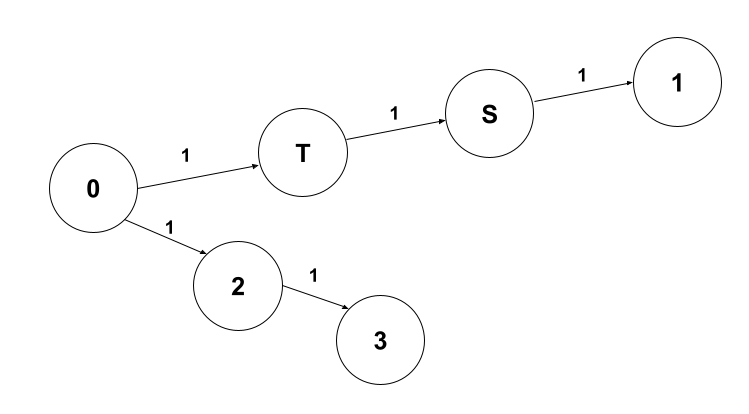
\includegraphics[height=7cm]{assn 4.png}

In this case, in predecessors node 1 would point to node S, then node S would point to node T, then node S would point to node 0. We want to update predecessors so that node 0 is pointing 1. To do so, we must traverse predecessors backwards so that we update node T before updating node 0. This is why we reverse topologically sort the graph.

\item Given node $n \in \Nodes$, provide an algorithm that can compute the shortest path (in terms of the sum of the weights of edges on the path) from node $n$ to any other node $m$ in $\OOG{W\abs{\Nodes} + \abs{\Edges}}$.

We must start by creating G' where every node is split into a chain of nodes as long as the biggest outgoing edge it has. These are all temporary nodes T, where there is an edge of weight 1 between them. This whole chain of temporary nodes represents the original node and any outgoing edge will come off one of those temporary nodes based on its weight. An example image is shown below to explain.

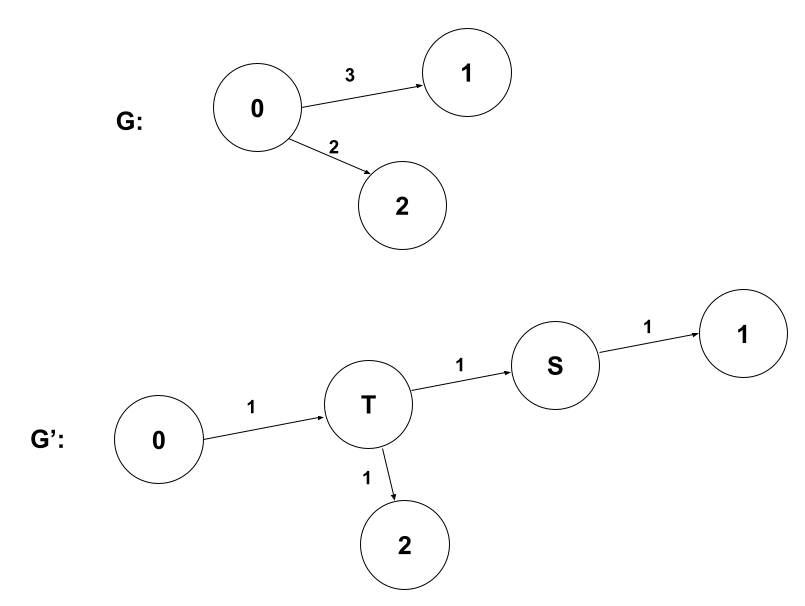
\includegraphics[height=10cm]{assn 4_3.png}

After this is done, we can perform the same algorithm as in 4.2.

\begin{myalgo}{\AName{SSSP}($G, s$)}
  \STATE create G'($N'$, $\Edges'$)
  \STATE $predecessors = \{n -> \:? \:|\: n \in \mathcal{N'}\}$
  \STATE $predecessors[s] = s$
  \STATE $Q =$ a queue
  \STATE $ENQUEUE(Q, s)$
  \WHILE{$!EMPTY(Q)$}
    \STATE $n = DEQUEUE(Q)$
    \FORALL{ $(n,m) \in \Edges'$}
      \IF{$predecessors[m] = \: ?$}
        \STATE $predecessors[m] = n$
        \STATE $ENQUEUE(Q, m)$
      \ENDIF
    \ENDFOR
  \ENDWHILE

  \STATE Reverse topological sort predecessors (sorted by edges in G')
  \STATE Go through all elements in topologically sorted predecessors and for anything pointing to a temporary node, make it point to the node nearest node in original N it is pointing towards.
  \STATE Remove all temporary nodes from $predecessors$

  \RETURN $predecessors$
\end{myalgo}

The graph representation used again is adjacency list representation.

This algorithm is the same as explained in 4.2 (please check 4.2 for correctness of what isn't explained here), however, we transform our graph G' in a different manner. This time, we must split all nodes into maximum $W$ nodes. This means that an upper bound for the number of nodes we will have is $W|N|$. Transforming graph G to G' will take $\OOG{N}$ time since we must go through every node once to split it.

This algorithm is BFS but with $W|N|$ nodes meaning that the time complexity of this algorithm will be $\OOG{W\abs{\Nodes} + \abs{\Edges}}$.


\end{questions}
For each question, explain why your algorithm is correct, why your algorithm achieves the stated complexity, and which graph representation you use.
\end{problem}

\SUBMITMSG{}
\DEFAULTGRADING{}

\end{document}